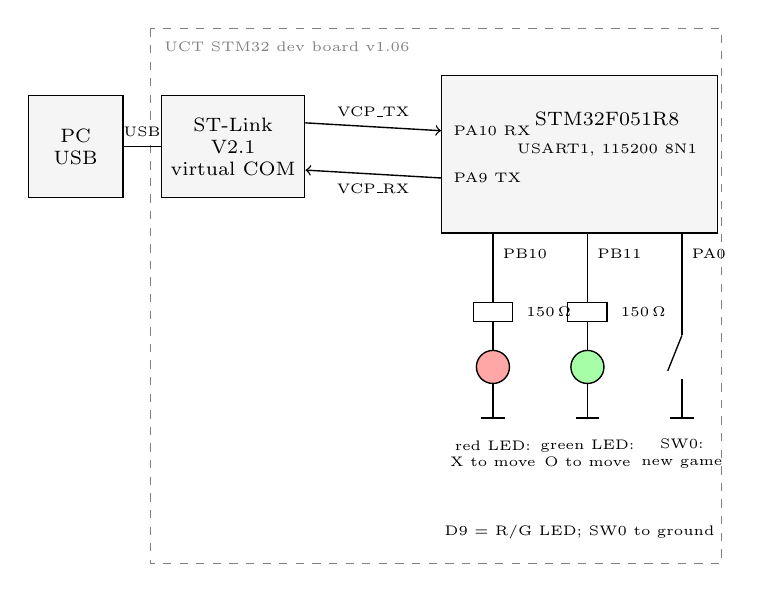
\begin{tikzpicture}[font=\scriptsize,line width=0.5pt,
  box/.style={draw,align=center,fill=gray!8},
  res/.style={draw,minimum width=0.5cm,minimum height=0.24cm,fill=white,inner sep=0pt}]
  \draw[dashed,gray] (1.55,1.5) rectangle (8.8,-5.3);
  \node[anchor=north west,font=\tiny,gray] at (1.6,1.45) {UCT STM32 dev board v1.06};
  \node[box,minimum width=1.2cm,minimum height=1.3cm] (pc) at (0.6,0) {PC\\USB};
  \node[box,minimum width=1.6cm,minimum height=1.3cm] (stl) at (2.6,0) {ST-Link\\V2.1\\virtual COM};
  \node[box,minimum width=3.5cm,minimum height=2.0cm] (mcu) at (7.0,-0.1) {};
  \node at (7.35,0.35) {STM32F051R8};
  \node[font=\tiny] at (7.35,-0.05) {USART1, 115200 8N1};
  \draw (pc.east) -- node[above,font=\tiny]{USB} (stl.west);
  \draw[->] ([yshift=0.3cm]stl.east) -- node[above,font=\tiny]{VCP\_TX} ([yshift=0.3cm]mcu.west);
  \draw[<-] ([yshift=-0.3cm]stl.east) -- node[below,font=\tiny]{VCP\_RX} ([yshift=-0.3cm]mcu.west);
  \node[font=\tiny,anchor=west] at ([xshift=1pt,yshift=0.3cm]mcu.west) {PA10 RX};
  \node[font=\tiny,anchor=west] at ([xshift=1pt,yshift=-0.3cm]mcu.west) {PA9 TX};
  % LED and button
  \foreach \x/\pin in {5.9/PB10,7.1/PB11,8.3/PA0} {
    \draw (\x,-1.1) -- (\x,-1.9);
    \node[font=\tiny,anchor=south west] at (\x,-1.55) {\pin};
  }
  \foreach \x/\col/\cap in {5.9/red/{red LED:\\X to move},7.1/green/{green LED:\\O to move}} {
    \node[res] at (\x,-2.1) {};
    \draw (\x,-1.9) -- (\x,-1.97); \draw (\x,-2.23) -- (\x,-2.6);
    \node[draw,circle,minimum size=0.42cm,inner sep=0pt,fill=\col!35] at (\x,-2.8) {};
    \draw (\x,-3.01) -- (\x,-3.45);
    \draw (\x-0.15,-3.45) -- (\x+0.15,-3.45);
    \node[font=\tiny,align=center] at (\x,-3.9) {\cap};
  }
  \node[font=\tiny,anchor=west] at (6.2,-2.1) {150\,$\Omega$};
  \node[font=\tiny,anchor=west] at (7.4,-2.1) {150\,$\Omega$};
  % button to ground
  \draw (8.3,-1.9) -- (8.3,-2.4); \draw (8.3,-2.4) -- (8.12,-2.85); \draw (8.3,-2.95) -- (8.3,-3.45);
  \draw (8.15,-3.45) -- (8.45,-3.45);
  \node[font=\tiny,align=center] at (8.3,-3.9) {SW0:\\new game};
  \node[font=\tiny] at (7.0,-4.9) {D9 = R/G LED; SW0 to ground};
\end{tikzpicture}
